\documentclass[a4paper]{article}
\usepackage[utf8]{inputenc}
\usepackage[russian]{babel}
\usepackage{listings}
\usepackage[a4paper]{geometry}
\usepackage{indentfirst}
\usepackage{graphicx}
\usepackage{caption}
\usepackage{float}
\usepackage{amssymb}
\usepackage{url}
\usepackage{physics}

\begin{document}

\title{Отчёт по курсу <<Высокопроизводительные параллельные вычисления на кластерных системах>>.}
\author{Владислав Соврасов\\ аспирант гр. 2-о-051318}
\date{}
\maketitle

\section{Постановка задачи}

Требуется получить параллельную версию солвера MIDACO \cite{midacoURL}, которая
бы эффективно работала как на распределённых системах, так и на системах с общей памятью.

MIDACO (Mixed Integer Distributed Ant Colony Optimization) предназначен для решения
глобальной оптимизации как с дискретными, так и с непрерывными параметрами.

Будем рассматривать задачу глобальной оптимизации в непрерывном многомерном пространстве:
\begin{displaymath}
\label{eq:task}
\varphi(y^*)=\min\{\varphi(y):y\in D\},D=\{y\in \mathbf{R}^N:a_i\leqslant x_i\leqslant{b_i}, 1\leqslant{i}\leqslant{N}\}
\end{displaymath}

В качестве тестовых задач для измерения производительности рассматривались 100
четырёхмерных задач вида (\ref{eq:task}), полученных генератором GKLS \cite{GKLS}.

\section{Реализация}

Авторы MIDACO предлагают использовать довольно простую схему распараллеливания (рис. \ref{fig:midaco}):
интерфейс их метода устроен таким образом, что на каждой итерации позволяет
получить заданное количество точек, в которых необходимо вычислить значение целевой
функции. Вычисление во всех точках могут быть проведены параллельно. В практических задачах глобальной оптимизации
целевая функция, как правило, достаточно трудоёмка, поэтому данная схема имеет смысл.

Вместе с исходным кодом MIDACO предоставляются примеры распараллеливания вычисления целевой функции как на распределённой,
так и на общей памяти. Они имеют ряд недостатков:
\begin{itemize}
  \item нет примера, сочетающего в себе смешанную модель распараллеливания на
  общей + распределённой памяти;
  \item все примеры написаны на языке C таким образом, что в них нет чётко выделенного интерфейса для солвера,
  который бы обеспечивал удобство использования;
  \item в распределённой версии для передачи многомерных точек на другие узлы используются
  MPI-операции Send/Receive, в то время как описанная схема идеально подходит под использование
  Scatter/Gather и может быть эффективнее реализована с их помощью. Эта проблема особенно актуальна в режиме смешанного
  распараллеливания, когда на каждый узел вместо одной точки будут пересылаться несколько.
\end{itemize}

\begin{figure}[H]
  \center
  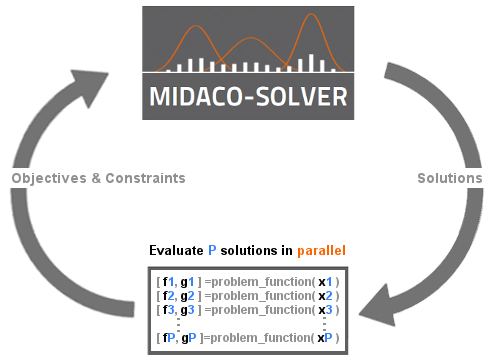
\includegraphics[width=0.5\textwidth]{parallel_loop.png}
  \caption{Схема распараллеливания в MIDACO}
  \label{fig:midaco}
\end{figure}

Учитывая все перечисленные недостатки публично доступной параллельной версии MIDACO, была
подготовлена собственная реализация, предоставляющая более удобный C++ интерфейс к солверу,
реализующая параллельное вычисление целевой функции на различных узлах и на различных процессорах в
рамках одного узла, использующая при этом эффективные групповые операции Scatter/Gather.
Часть исходного кода приведена в секции \ref{sec:source}.

\section{Результаты}

Все вычислительные эксперименты проводились на узлах суперкомпьютера <<Лобачевский>>, каждый узел которого
имеет 16 вычислительных ядер. В экспериментах было задействовано до 12 узлов. Таким образом, максимальное
количество задействованных вычислительных ядер достигало 192.

В каждом эксперименте решались 100 четырёхмерных задач, полученных генератором GKLS.
Измерялось количество обращений к целевой функции и время решения каждой задачи.
С целью имитации трудоёмких целевых функций в вычисление каждой функции вносилась искусственная задержка,
равная в различных экспериментах 0.1, 0.5 или 1мс. Задержка реализована в виде дополнительной
нагрузки по вычислению некоторых элементарных функций. Объём вычислений подбирался так, чтобы они занимали заданное время.

Во всех экспериментах считается, что тестовая задача решена, если метод оптимизации провёл очередное испытание \(y^k\) в
\(\delta\)-окрестности глобального минимума \(y^*\), т.е. $\left\|y^k-
y^*\right\|\leqslant \delta = 0.01\left\|b-a\right\|$, где \(a\) и \(b\) --- левая и правая границы гиперкуба из (\ref{eq:task}).
Если указанное соотношение не выполнено до истечения лимита на количество испытаний, то задача считается нерешённой.
Максимальный лимит на количество испытаний установлен раным $250\cdot 10^3$

На рис. \ref{fig:speedup_nodes} приведён график ускорения по времени ($S_p=\frac{t_1}{t_p}$)
при различном количестве узлов и потоков на один узел, а также всех рассматриваемых значениях задержки в
целевой функции. Из графика видно, что ускорение достигает максимальных значений при задержке 1мс, т.к.
накладные расходны на передачу данных становятся меньше по сравнению с временем вычисления целевых функций.
Использование 16 ядер на каждом узле также приносит значительное ускорение, по сравнению с использованием одного
ядра на узел. При увеличении количества узлов ускорение линейно нарастает.

\begin{figure}[H]
  \center
  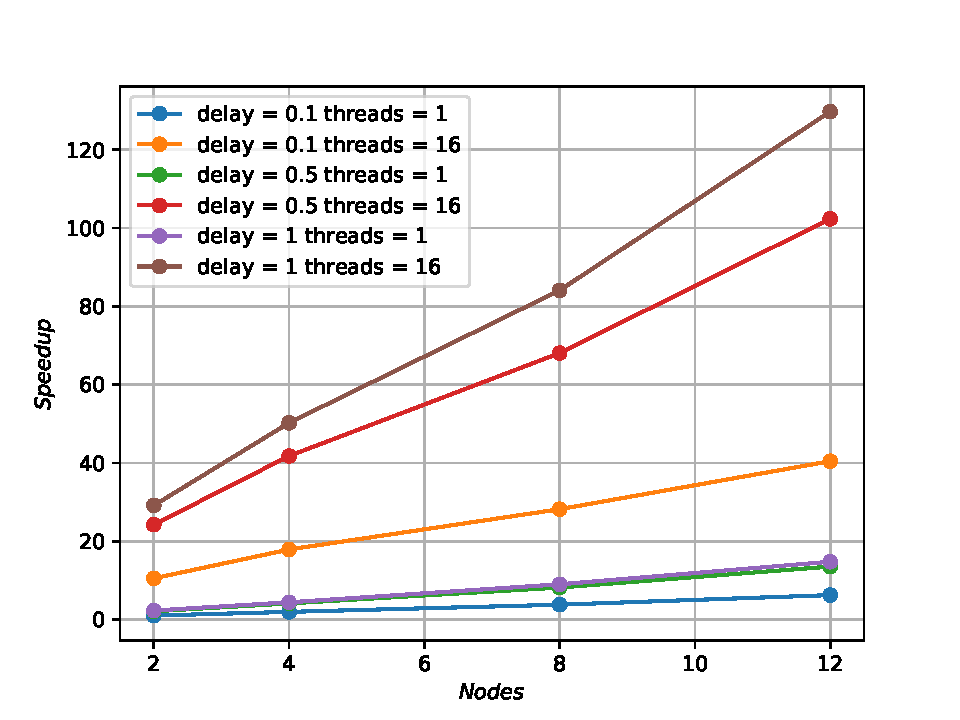
\includegraphics[width=0.75\textwidth]{gpu_mpi/gklsh4d/speedup_nodes.pdf}
  \caption{Графики полученного ускорения по узлам в зависимости от трудоёмкости вычисления целевой функции}
  \label{fig:speedup_nodes}
\end{figure}

В таблице \ref{tab:speedup} приведено количество итераций метода в каждой из конфигураций,
количество решённых задач, а также ускорения по времени $S_p$ и по итерациям $S_p^i=\frac{iters_p}{iters_1}$.
$S_p^i$ является верхней границей для $S_p$, т.к. в лучшем случае каждая параллельная итерация
занимает столько же времени, сколько последовательная. Параллельный метод делает меньше итераций,
за счёт того, что на каждой из них проводит больше испытаний, однако ускорение по итерациям может быть в некоторых случаях
меньше количества вычислительных устройств из-за избыточности по испытаниям,
характерной для методов параллельной глобальной оптимизации. Согласно таблице \ref{tab:speedup},
ускорение по времени довольно близко к ускорению по итерациям при малом количестве вычислительных
устройств. С ростом количества узлов и потоков $S_p$ начинает заметно отставать от $S_p^i$, однако
при этом сохраняется приемлемое соотношение между ними. Также стоит заметить, что метод оптимизации,
реализованный в MIDACO, с ростом количества испытаний на итерацию решает меньше задач за отведённое число испытаний.
Эта ситуация происходит при использовании схем распараллеливания (4, 16), (8, 16) и (12, 16).

\begin{table}[H]
\begin{center}
\caption{Показатели ускорения по времени и по итерациям при задержке 1мс}
  \begin{tabular}{|l|{c}|{c}|{c}|{c}|{c}|{c}|{c}|{c}|{c}|{c}|}
    \hline
    Узлы, потоки &  $S^i_p$ & $S_p $ &  & Итерации & Решено задач \\
  \hline
  1, 1   & 72068 & 132.5s & & 72068 & 71 \\
  1, 16  & 16.7  & 14.4   & & 4304 &  70 \\
  2, 1   & 2.7   & 2.3    & & 27128 & 73 \\
  2, 16  & 32.0  & 29.1   & & 2254 & 73  \\
  4, 1   & 4.5   & 4.4    & & 15980 & 75 \\
  4, 16  & 57.0  & 50.2   & & 1264 & 66 \\
  8, 1   & 10.3  & 9.0    & & 9853 & 83 \\
  8, 16  & 93.1  & 84.1   & & 774 & 57 \\
  12, 1  & 16.0  & 14.8   & &6022 & 86 \\
  12, 16 & 183.2 & 129.7  & & 393 & 53 \\
  \hline
  \end{tabular}
  \label{tab:speedup}
\end{center}
\end{table}

\section{Исходный код}
\label{sec:source}
Полная версия кода доступна по ссылке \url{https://github.com/sovrasov/midaco-mpi-cpp}.
\lstinputlisting[language=C++, numbers=left]{../src/midaco_mpi.cpp}

\begin{thebibliography}{}

\bibitem{midacoURL}
\url{http://www.midaco-solver.com}

\bibitem{GKLS}
\url{http://wwwinfo.deis.unical.it/yaro/GKLS.html}

\end{thebibliography}

\end{document}
